\pagebreak
\subsection{License}
Gpvdm comprises of three independent components, gpvdm gui, gpvdm core and gpvdm data.  In general everything is under the MIT license except the Python GUI which I have released under GPL v2.0. Details can be found \href{https://github.com/roderickmackenzie/gpvdm/blob/main/LICENSE.md}{here}.

\subsection{Using gpvdm in industrial/academic work}
\label{sec:using_gvpdm}
You are free to use gpvdm in industrial/academic work. In fact, I'm super happy if you use it in your work, papers or books. However, the following further conditions apply:\\\\
1. If you use gpvdm to generate results, then clearly say so in your work. This can be as simple as one sentences saying: "we used gpvdm to perform the simulations" \\\\
2. If you publish a book, paper or thesis where gpvdm has been used you must cite at least three papers associated with the model.  To find out which papers to cite, click on the area indicated in red in figure \ref{fig:cite_me} when using the model.   You are free to choose which papers to cite but PLEASE do not cite the manual. I can't include the manual in paper lists when applying for funding.\\
\\
I ask you to do this because citations are an easy way to demonstrate that people are using gpvdm. Demonstrating use is key to finding money/people to continue the development of gpvdm.  So by doing this you are guaranteeing the future of gpvdm and it's continued availability for others.  Thank you!

\begin{figure}[ht!]
\centering
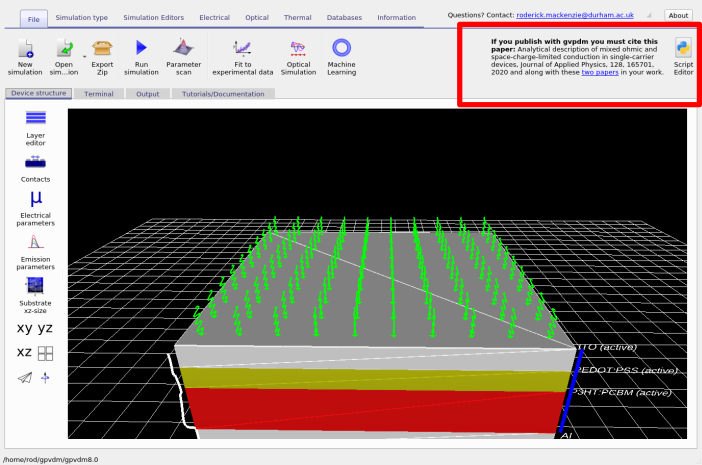
\includegraphics[width=\textwidth]{./images/cite_me2.png}
\caption{If you click on the area indicated by the red box, the model will tell you which papers should be cited.}
\label{fig:cite_me}
\end{figure}

